\usepackage{graphicx}
\graphicspath{ {images/} }
\section{OpenNebula}
\url{https://opennebula.org/} \\ 
   
OpenNebula is a useful tool that enables seamless management and control of different cloud systems.
The tools can be used for public, private or hybrid cloud implementations.
The tool can be used to virtualize data centers and also to obtain solution for cloud infrastructure.
The tool can be used on top of existing cloud infrastructure.
OpenNebula project started on 2005 and currently the product is available as an open-source under Apache license. \\
‘‘The toolkit includes features for integration, management, scalability, security and accounting.
It also claims standardization, interoperability and portability, providing cloud users and administrators with a choice of several
cloud interfaces (Amazon EC2 Query, OGF Open Cloud Computing Interface and vCloud) and hypervisors
(Xen, KVM and VMware), and can accommodate multiple hardware and software combinations in a data center ’’
~\cite{hid-sp18-417-opennebula-wiki}.\\

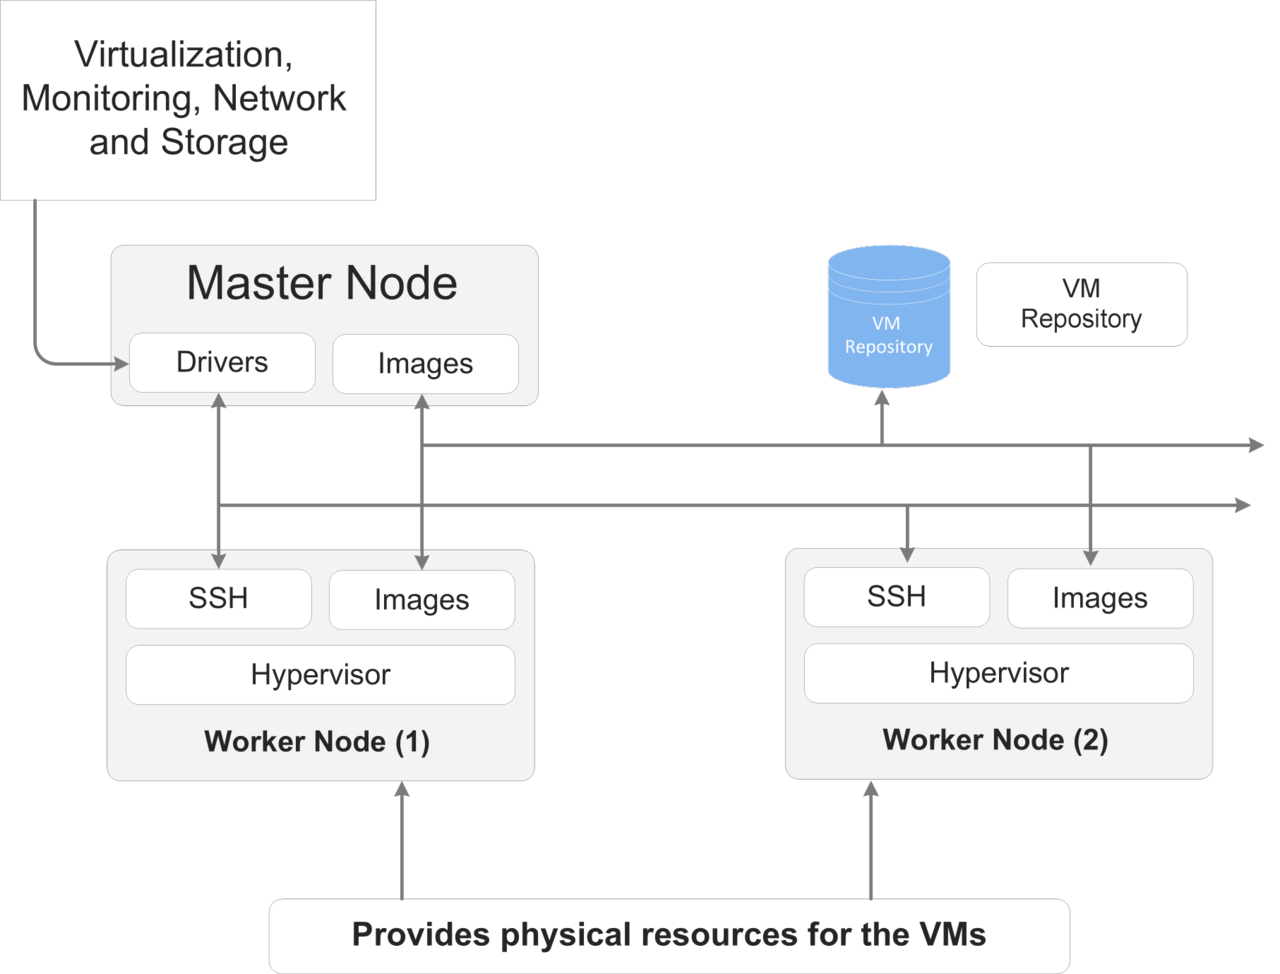
\includegraphics{hid-sp18-417-opennebula}
\begin{center}
OpenNebula Deployment Model ~\cite{hid-sp18-417-opennebula-deployment} 
\end{center}

The OpenNebula deployment needs :
\begin{itemize}
\item        A client node
\item        A hypervisor
\item        A data storage system
\item        Physical network
\end{itemize}

Due to its long steady growth, the tool is being used by customers in various industries ranging from telecom to education.
The wide range of customer base is helpful in providing a solid support system to the new and existing users as well as continuous
feedback becomes vital in the research and growth of the project. 

